\documentclass{article}
\usepackage[utf8]{inputenc}
\usepackage{graphicx}

\title{\textbf{Electronic Voting Machines in Indian Elections}
\linebreak A Case Study}
\author{Animesh Singh}
\date{May 2018}

\begin{document}

\maketitle

\begin{abstract}
This document pin points the various flaws in the current EVM system used for voting in India and solves those problems by proposing a new design. Section 1 provides an introduction to the problem and motivation to propose solutions. Section 2 discusses the stakeholders of the problem followed by Section 3 which is the Needs Analysis where we have discussed the basic set of properties that needs to be satisfied by an EVM. Section 4 mention the relaxation conditions assumed for the proposal and Section 5 illustrates the various basic design foundations available. Section 6 proposes a functional design based on Section 5.1 and Section 7 based on section 5.2. Section 8 provides methods for testing the structure followed by Section 9 which contains References.
\end{abstract}

\section{Introduction}

Fair and accurate elections are vital for a healthy democracy. India being the world's largest democracy, organizing the most wide-scale elections on the planet is a daunting task for the Election Commission of India. Any voting system carries with it some risks. Electronic voting systems introduce whole new classes of risks in addition to the general ones.\par
Elections in India are conducted almost exclusively using electronic voting machines. EVMs have been praised for their simple design, ease of use, and reliability, but they have also been criticized following reports of election irregularities and lack of rigorous, independent security evaluation.


\section{Stakeholders}

I identify the following stakeholders for the given design problem.

\subsection{Primary Stakeholders}

\begin{enumerate}  
\item Voters - The common \emph{junta} is (arguably) the most vital stakeholder in the entire election process because this entire ruckus is caused to provide better governance for the people (\emph{right?}).
\item Candidates - The candidates standing for the elections are also primary stakeholders in the process because ultimately its their fate that is being decided by the elections.
\item Election Commission Employees - They are primary stakeholders as well because they are an inseparable part of the election process. They sit through the entire operation, assist the voters in case of problem and handle the candidates' queries. 
\end{enumerate}

\subsection{Secondary Stakeholders}

\begin{enumerate}  
\item Political Party \emph{Karyakarta}s - They are stakeholders as well because they mobilize support for the party day in and day out. Election results are an indirect result of their work.
\item Political Parties - They are the ones benefiting from the victory of a said candidate.
\item Election Commission of India - They are held responsible for the entire election process. They would be credited with the success or failure of the operation.
\item India as a Nation - It is the fate of the nation that is being decided ultimately.
\end{enumerate}

\section{Needs Analysis}

\subsection{Transparency}

Transparency is a key principle for credible elections. A transparent election process is one in which each step is open to scrutiny by stakeholders (political parties, election observers and voters alike), who are able to independently verify the process is conducted according to procedures and no irregularities have occurred. Providing transparency in an election helps establish trust and public confidence in the process, as voters have a means to verify the results are an accurate reflection of the will of the people.\par
Electronic voting and counting technologies pose a challenge to ensuring transparency, since many visually-verifiable steps in a traditional election (such as how ballots were marked) are automated inside a machine and, therefore, cannot be seen by the voter and others. In such circumstances, particular efforts must be made to provide transparency in each step of the process. 

\subsection{Secrecy}

The secrecy of the vote is seen as one of the fundamental principles required in the conduct of democratic elections. Failure to secure the secrecy of the vote opens the possibility for voters to prove how they have voted, facilitating voter coercion and vote buying. Both of these practices undermine the free expression of the will of the voter and the possibility for election results to reflect the will of the voters.\par
If implemented properly, the paper-based system of voting effectively protects the secrecy of the vote. In the case of electronic counting, the same protections that currently exist for the hand counting of paper ballots should be applied. Electronic voting, however, introduces a number of additional ways secrecy can be violated. Voting machines record the choices cast on them by voters, and these votes may be recorded in the order in which they are cast with a timestamp. This means if someone knows the order in which voters cast their ballots on a voting machine or the time at which a voter cast their ballot and has access to the record of voting on the machine, they could determine the choices made by each voter.

\subsection{Accountability}

Elections are the primary means by which voters hold those elected to office accountable. While elections create an accountability mechanism, there must also be accountability within an election process if it is to be genuine. Accountability in an election process ensures those who conduct elections do so in compliance with the election legislation and relevant procedures, and in a manner that promotes the integrity of the process. \par
Generally, elections are conducted by election management bodies (EMBs). Within EMBs it is critical that responsibilities are clearly defined, including who has authorization to take specific actions or decisions. Officials at all levels of election administration must be responsible for their actions and decisions, and must be held accountable should they fail in their duties. Disciplinary measures and penalties must be defined for such instances, including the possibility of criminal liability for serious offenses.

\subsection{Security}

The security of the electoral process is critical for all elections. There are always points at which those wishing to manipulate the system could attempt to manipulate vote data. System security is especially important for electronic voting and counting systems, which may introduce new vulnerabilities into an election process. These vulnerabilities include external security threats to the security of the system, as well as internal threats of manipulation by those with official access to the system. These technologies are inherently less transparent than paper ballots, where all steps in the voting and counting process are observable. If electronic voting and counting systems are to be trusted by electoral stakeholders, it is important that the security challenges presented by the use of the technology are understood. Mechanisms must be in place to mitigate these security challenges, and any security breaches should be easily identified.

\subsection{Integrity}

One of the fundamental principles elections must comply with is that they must accurately reflect the will of the voters. The integrity of the electoral process also has implications for other related issues, as discussed later in the section on trust.\par
The integrity of the process when using electronic voting and counting technologies is a particular challenge because of the nature of these technologies. With traditional paper balloting and hand counting, the entire process is not only clearly visible to those observing it, but it is also easily understandable to the average voter. The ballot box can be shown to be empty at the start of voting by polling staff, then sealed, observed in the polling station to ensure that only legitimate voters are putting in ballots, and at the end of voting the seal can be broken and the ballots counted in full view of observers. This overall transparency and simplicity of the process makes it relatively easy to observe the process and identify errors in the system if and when they occur. While political party and candidate agents, observers and the media perform a monitoring function, they also carry out a verification function to ascertain whether the process leads to an accurate reflection of the will of the voters.

\subsection{Auditable}
A great strength of the paper balloting system is that if the results of an election are challenged then the ballots can be recounted to check the result. Many electronic voting machines have no such possibility for auditing and checking the results of an election. The ability to audit and check is an important feature of building trust in the electoral process and increasing acceptance of the results.

\section{Relaxation Conditions}

I identify the following relaxation conditions for the given design problem.
\begin{enumerate}  
\item Non-repudiation and maintaining the anonymity of the voter are somewhat conflicting needs and I prioritize secrecy of the voter in our design.
\item I assume that the system would be in the correct working condition for the process. This implies that there would be no cases of coercion due to irregular display of option candidates or jamming of buttons etc.
\item I assume that the system will be manufactured in a trustworthy facility. The initial make of the system is not biased and if there is an attempt to tamper with it (through various kind of possible attacks), a mechanism disables the voting machine altogether.
\end{enumerate}


\section{Solution Designs for Functional Structure}

\subsection{Direct Recording Electronic (DRE) System}

Often referred to as electronic voting machines (EVMs), DRE systems use a keyboard, touch-screen, mouse, pen or other electronic device to allow a voter to record his or her vote electronically. DREs are used in non-remote, supervised locations (polling stations). The DRE system captures the voter’s choices and stores an electronic record of their vote in the machine. The data captured by each individual DRE unit is then transmitted by either electronic means (i.e., Internet, cellular network or memory card) or manually (i.e., by printing the results from each machine and tabulating them) to capture the total number of votes cast for specific parties or candidates. DRE systems may or may not produce a paper record to allow the voter to verify their voting choices. This paper record, also called a voter verified paper audit trail (VVPAT), has been implemented in multiple ways in different countries.
DREs with VVPATs are perceived to have an advantage over DREs without VVPATs, because paper trails provide greater transparency to the voter, which can engender greater trust. DRE voting without VVPATs, which is a form of “black box voting”, does not provide sufficient means for voters and stakeholders to verify votes have been accurately recorded. DREs with VVPAT provide election management bodies (EMBs) and those who provide oversight with the potential to audit the results or conduct a meaningful recount. However, DREs with VVPATs also introduce greater technological complexity into the process, which may result in greater challenges for EMBs in terms of reliability of the machine, training for staff and sustainability of the overall system. 
DREs can be confusing for voters who are not familiar or comfortable with information technology (IT). However, in some contexts, voters may benefit from a streamlined presentation of ballots on DREs in complicated voting systems – with or without VVPAT – where a paper ballot design may lead to a significant number of spoilt and invalid ballots.

\subsection{Electronic Ballot Printers (EBPs)}
 
Dr. Rebecca Mercuri proposed this system that is based on EBPs which are similar to DREs, in that the voter uses a DRE-type interface for the act of making voting choices. However, unlike DREs, an EBP does not store vote data. Instead, it prints out a paper receipt or produces a token containing the voting choice(s). The voter then takes this receipt or token and places it into the ballot box, which may be electronic and automatically count the vote. 
EBPs are considered easier to understand and more user-friendly for the voter than DREs, as they split the actions of marking the voter’s choice and casting the ballot in the same way a voter marks and casts a ballot in traditional paper voting. The first machine (ballot printer) only marks the voter’s choice, but does not record the vote, while the second machine (ballot scanner or “electronic ballot box”) only records and tallies the votes. Like the DREs with a VVPAT, the voter can verify their vote, either on a printed paper ballot or by inserting the ballot token into another voting machine. There is the possibility of a recount of the paper receipt or token if the electronic results are challenged or audited. However, because they involve two separate machines, EBP systems may entail higher costs, require greater IT capacity from EMBs and encounter more challenges to ensuring sustainability than other systems.
 
 
\subsection{Optical Mark Recognition (OMR)}
OMR counting machines combine aspects of paper ballot voting with electronic counting. The voter uses a pen or pencil to mark his or her choices (usually by filling in an oval or connecting an arrow) on a special machine-readable paper ballot. The ballot is then read by an OMR machine that tallies votes using the marks made by the voter. There are two methods used to tally votes using an OMR system. The tallying can be done at the polling station with the voter feeding the ballot into the machine, or votes can be tallied at a central/regional counting facility where votes from more than one polling station are counted. 
OMR systems provide greater ability for recounts than DREs without VVPAT. Generally, OMR systems cost less than DREs and may put less strain on EMBs in terms of sustainability of the systems. On the other hand, these systems entail significant focus on details such as ballot design, type of ink used, paper stock thickness and other factors that may inhibit the ability of OMR machines to accurately count votes. OMR machines are always used in a supervised, non-remote location.
 
\subsection{Internet Voting System}
In an Internet voting system, the voter casts his or her vote using a computer with access to the Internet. Internet voting generally takes place in an unsupervised, remote location, from any computer that has Internet access, such as a voter’s home or work. It can also take place in supervised, non-remote locations if, for example, electoral authorities provide Internet kiosks at polling stations. \par
Convenience and greater access are the two key benefits cited for a move to Internet voting. In terms of access, Internet voting is perceived to provide access to specific populations that may have difficulty in voting at polling stations, e.g. persons with disabilities and eligible voters living outside a country. However, Internet voting from unsupervised locations requires voting systems to place a greater emphasis on voter authentication to avoid impersonation, and also elicits concerns about the secrecy of the ballot. Internet voting also raises security concerns with regard to hacking into the system or other ways of corrupting data. Similar to DREs without VVPAT, Internet voting also raises questions about verifiability, may not allow recounts and presents challenges for adjudication of electoral complaints. Finally, transparency in Internet voting systems may be compromised to an even greater extent than with DREs. Such challenges are not beyond solution, but to date remain significant.


\section{Proposed Functional Structure - 1}

I propose several changes to the current model of the EVM to satisfy our requirements (through need analysis). It is still based on the DRE mechanism.

\begin{figure}[h!]
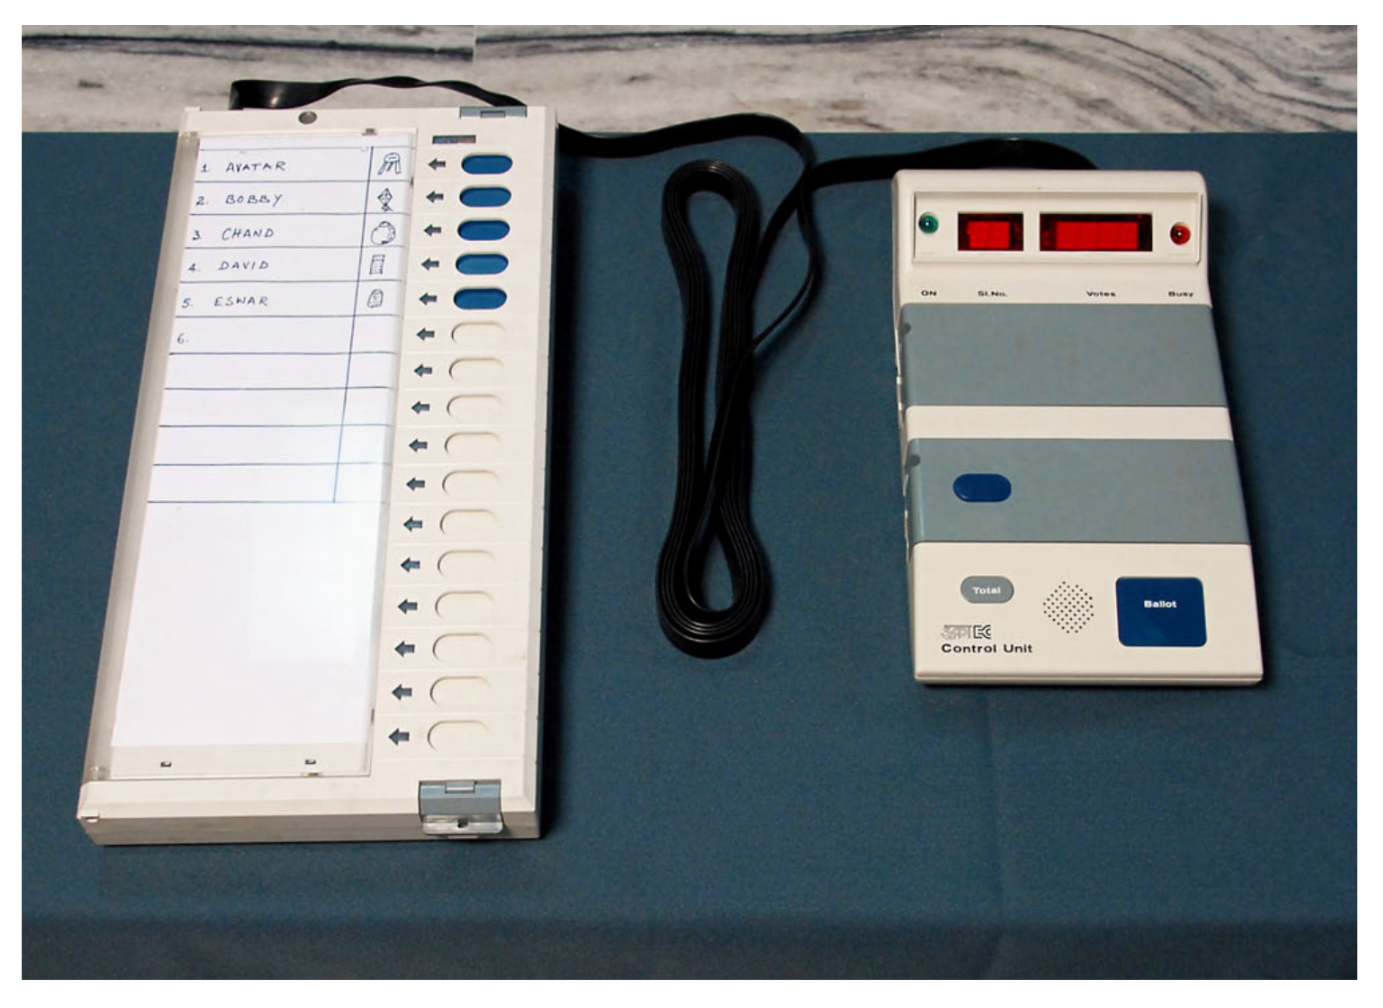
\includegraphics[width=0.5\textwidth]{evm1.png}
\centering
\caption{EVMs consist of a ballot unit used by voters (left) and a control unit operated by poll workers (right) joined by a 5-meter cable. Voters simply press the button corresponding to the candidate of their choice.}
\end{figure}


\begin{figure}[h!]
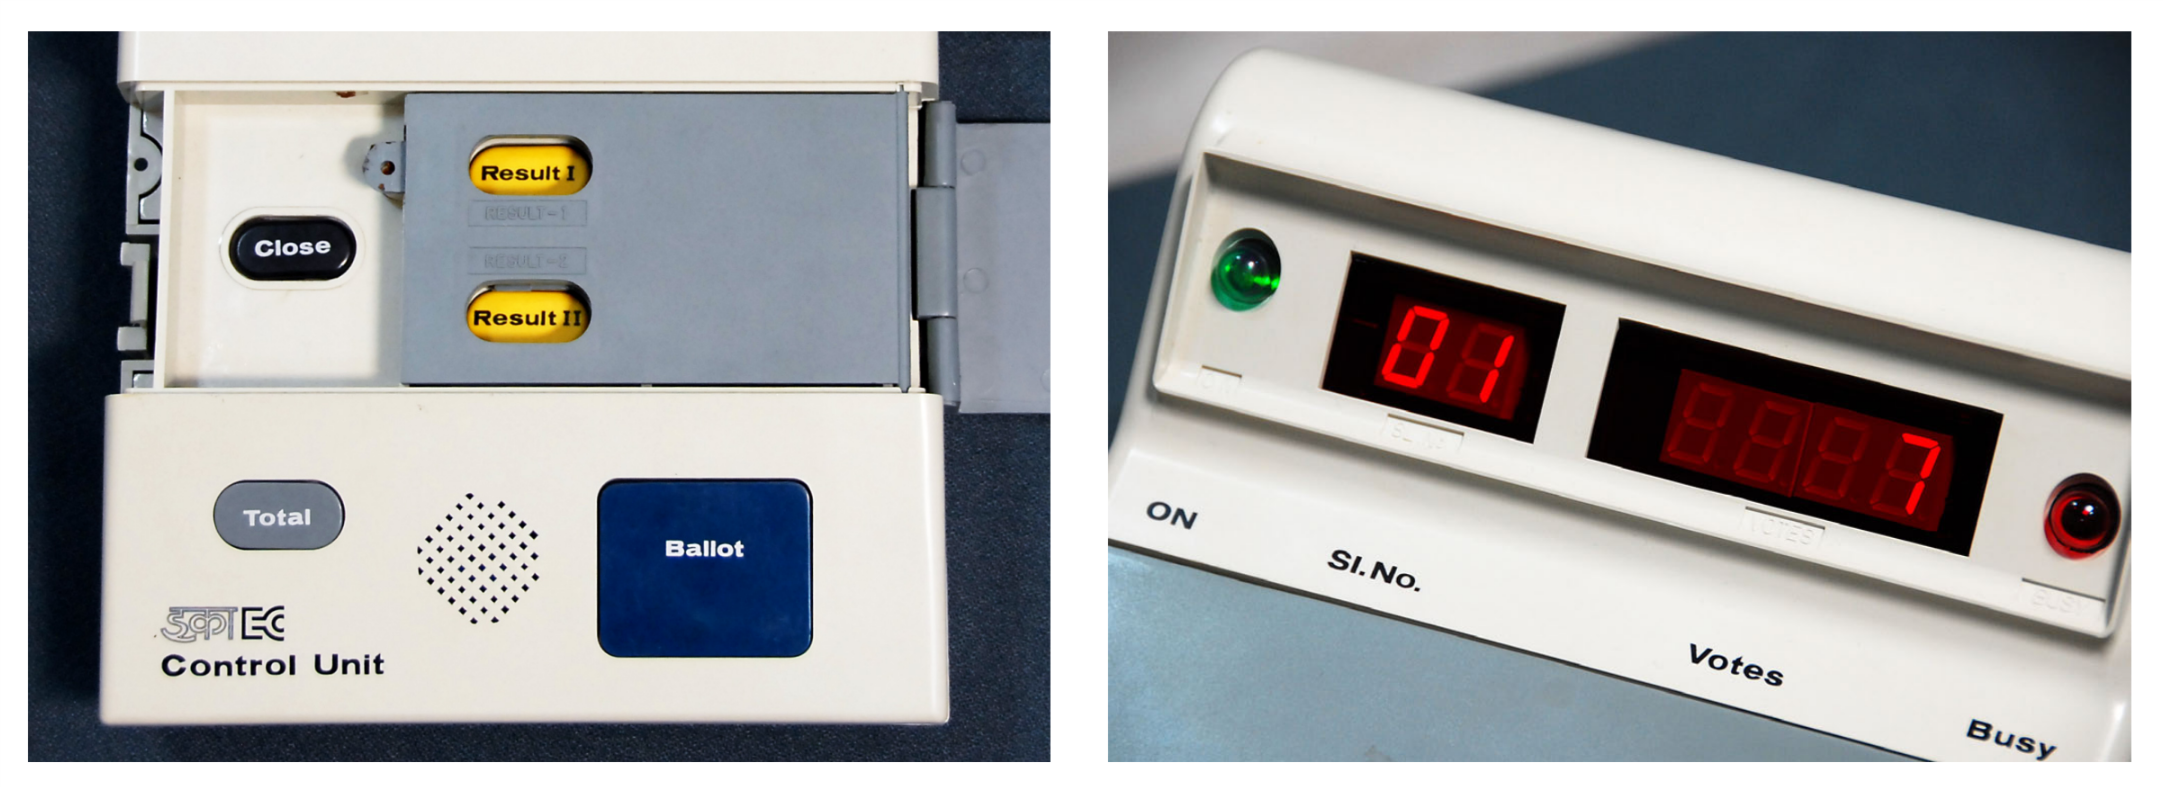
\includegraphics[width=1\textwidth]{evm2.png}
\centering
\caption{Counting Votes - The EVM records votes in its internal memory. At a public counting session, workers remove a seal on the control unit and press the result i button (left) to reveal the results. The machine sequentially outputs the number of votes received by each candidate using a bank of 7-segment LEDs (right). Here, candidate number 01 has received 7 votes.}
\end{figure}


The controller used in EVMs has its operating program etched permanently in silicon at the time of manufacturing by the manufacturer. No one (including the manufacturer) can change the program once the controller is manufactured. EVMs are powered by an ordinary 6 volt alkaline battery. This design enables the use of EVMs throughout the country without interruptions because several parts of India do not have power supply and/or erratic power supply. \par
In the current EVM structure, a candidate can know how many people from a polling station voted for him. This is a significant issue particularly if lop-sided votes for/against a candidate are cast in individual polling stations and the winning candidate might show favoritism or hold grudges against specific areas. I propose a unifier that can connect several balloting units and would display only the overall results from an Assembly or a Lok Sabha constituency instead of votes from individual polling stations. This can be done through control units electronically transmitting their results back to the Election Commission through a simple and unconditionally secure protocol, UMAC. Message authentication code based on universal hashing, or UMAC, is a type of message authentication code (MAC) calculated choosing a hash function from a class of hash functions according to some secret (random) process and applying it to the message. The resulting digest or fingerprint is then encrypted to hide the identity of the hash function used. As with any MAC, it may be used to simultaneously verify both the data integrity and the authenticity of a message. UMAC is specified in RFC 4418, it has provable cryptographic strength and is usually a lot less computationally intensive than other MACs. UMAC's design is optimized for 32-bit architectures; a closely related variant of UMAC that is optimized for 64-bit architectures is given by VMAC. The Indian EVMs are currently purposely designed as stand-alone units to prevent any intrusion during electronic transmission of results. Instead, the EVMs are collected in counting booths and tallied on the assigned counting day(s) in the presence of polling agents of the candidates. \par
Election Commission of India claims that for tampering of the EVMs, one needs physical access to EVMs, and pretty high tech skills are required. Given that EVMs are stored under strict security which can be monitored by candidates or their agents all the time, its impossible to gain physical access to the machines. I propose a BIST mechanism (Built-In Self Test) in which hardware and/or software is built into integrated circuits allowing them to
test their own operation, as opposed to reliance on external automated test equipment. The logic can involve a strong multi-level encryption. We can use hashing with the key as model no. of EVM, Date of Manufacturing and a random salt. This will be unique for each EVM and can be stored in a secure database. The untampered EVM's BIST should run some program on the circuit and should be able to generate a hash. If the hash is correct, an alarm / led is turned on. If it fails this test, it can be assured that the EVM is tampered and it shuts down. \par
A VVPAT system was introduced in the EVMs recently to counter the charges of tampering. These are sealed printers with a viewing window and a sealed box underneath. When a voter casts the vote by press of a key, a printed slip is generated which can be seen in the viewing window and is thereafter cut and deposited in the sealed box. Each vote registered by the machine therefore has a corresponding print and the results on the machine can be verified by counting the slips. To maintain anonymity of the voter, I propose a system of slip disposal that has a timestamp (for verifiability) initially. But, when the slip is put in the box, a mechanism snips off the timestamp region of the slip, and only the vote falls into the box. This ensures that no one can backtrack the vote through the timestamp to the said voter. In this process, this measure bends the non-repudiation condition. The current system also has vulnerabilities against hardware attacks like Clip-on Memory Manipulator Attack and Dishonest Display Attack. To rectify these, I assume that tampering original unbiased EVM leads to shut down of the system indicating such an attack. The vote count till then will still be preserved on memory.


\section{Proposed Functional Structure - 2}

I propose a new structure based on the EPB(Mercuri) Model. This system has all the benefits of a DRE system (ease of use, accessibility for impaired voters, rapid tabulation, etc.) yet still produces a human readable artifact for voter verification and recounts in the case of a challenge by one or more parties. A voter enters a booth and makes their selections on the DRE interface. The system then prints a human readable paper ballot inside a sealed transparent chamber. The separation prevents the voter from removing the ballot from the polling place and protects the ballot from accidental or intentional modification. The voter inspects the ballot for correctness and then it is deposited mechanically into a ballot box while the DRE records the ballot internally. If the ballot was not correct then the voter asks an election official to void the ballot and permit the voter to try again. Once the election is over, the DRE totals serve as the preliminary results until the paper ballots are scanned and tabulated. This method is also cost effective in the long run since elections no longer require blank ballots printed before each election. As an additional security measure each ballots can be digital signed with a cryptographic hash composed of information such as a precinct code, the voting machine serial number, and a choices on the ballot. The hash would provide an extra layer of verification to help determine if a set of ballots were tampered with before they were counted without violating voter privacy. While the method improves voter confidence and provides an audit trail, it does not prevent election fraud if the DRE is subverted. An election could still be rigged if the DRE randomly altered perhaps one ballot in 100. If a voter checked the ballot and noticed the change they would probably assume they entered the wrong choice. If they did not bother to check then the altered ballot would be counted as correct. Such and attack would be sufficient to swing close elections if applied in critical precincts. Hence, a proper DRE would be a pre-requisite (assumption) for this model.


\section{Testing of Functional Structure}

The following methods can be applied for testing proposed functional structure.
\begin{enumerate}  
\item Acceptance testing - This is a method of testing software that tests the functionality of an application performed on a system (for example software, batches of manufactured mechanical parts, or batches of chemical products) prior to its delivery. It would relate to the acceptance of the proposed model with respect to the requirements stated above. 
\item Performance testing - This test is used to determine the speed or effectiveness of a computer, network, software programme or device. This process can involve quantitative tests done in a laboratory, such as measuring the response time or the number of MIPS (millions of instructions per second) at which system functions. Qualitative attributes such as reliability, scalability and interoperability of the structure are also evaluated. Performance testing is often done in conjunction with stress testing. 
\item Stress testing - This is a form of testing used to determine the stability of a given system by testing beyond normal operational capacity, often to breaking point, in order to observe the results. Basically, putting excessive load on our proposed EVM. 
\item Security testing - This is a process to determine that an information system protects data and maintains functionality as intended. The six basic security concepts that need to be covered by security testing are: confidentiality of vote, integrity of vote, authentication of voter, authorization of voter, availability of vote and non-repudiation of vote. 
\item Usability testing - This is a technique used to evaluate a product by testing it on users. This can be seen as an irreplaceable usability practice, since it gives direct input on how real voters would use the system. 
\item Review of the source code - This is a systematic examination of the computer source code intended to find and rectify mistakes overlooked in the initial development phase, improving both the overall quality of the software and the developers’ skills. The code programmed in the non-programmable chip of the EVM must be absolutely error proof (I assume this is the case in our proposed system).
\end{enumerate}
These tests should be carried out by independent, authorised and competent agencies. 


\section{References}
\begin{enumerate}  
\item Ben Goldsmith: "Electronic Voting & Counting Technologies - A Guide to Conducting Feasibility Studies", International Foundation for Electoral Systems
\item Daniel P. Lopresti: "Electronic Voting: Problems & Solutions", Department of Computer Science & Engineering, Lehigh University, Bethlehem, PA
\item https://www.ndi.org/e-voting-guide/
\item I.V. Blankenship: "Trusting the Machine: Inherent Problems with Electronic Voting Systems", GIAC Security Essentials Certification (GSEC)
\item Scott Wolchok, Hari K. Prasad, Rop Gonggrijp and others: "Security Analysis of India’s Electronic Voting Machines"
\item Rajat Moona: "EVMs do stellar service as messengers of the people’s mandate, and every winning candidate loves them", The Times of India, 19 March 2017
\end{enumerate}


\end{document}
